\section{MAP \& MLE}
\begin{definition}[Maximum a posteriori (MAP)]
  \begin{displaymath}
    \MAP \triangleq \argmax_i\ \pi_i = \argmax_i\ p_i\ q_i
  \end{displaymath}
\end{definition}
\begin{definition}[Maximum Likelihood Estimation (MLE)]
  \begin{displaymath}
    \MLE \triangleq \argmax_i q_i \equiv \MAP \text{ assuming uniform priors }\ p_i = \frac{1}{N}\ \forall i
  \end{displaymath}
\end{definition}
More generally, if $X,Y$ are discrete RVs then
\begin{align*}
  \MAP\left[X \mid Y=y\right] &= \argmax_x\ \Prb\left(X=x \mid Y=y\right) \\
  \MLE\left[X \mid Y=y\right] &= \argmax_x\ \Prb\left(Y=y \mid X=x\right)
\end{align*}
\begin{itemize}
  \item Called detection because everything is discrete, i.e.,
    detection and classification are synonymous.
  \item MAP: which cause best explaisn the observed symptom.
  \item MLE: which cause best generates/induces the observed symptom.
\end{itemize}
\begin{example}[MAP/MLE Analysis of BSC]
  Consider a $\BSC\left(p\right)$ with $p < \frac{1}{2}$.
\end{example}
\begin{center}
  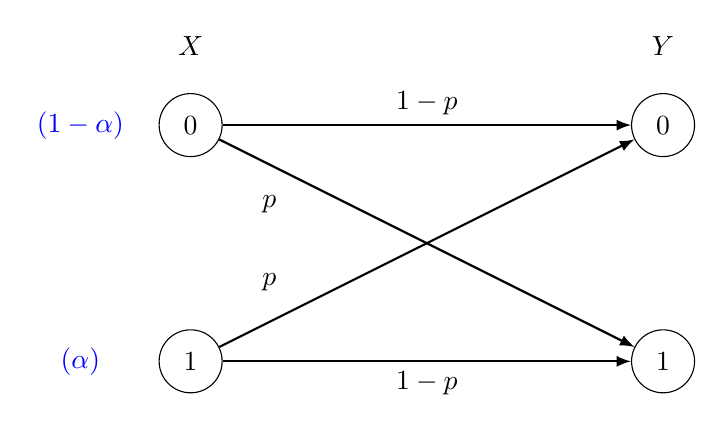
\begin{tikzpicture}[
      >=latex,
      node/.style={
        draw,circle,minimum size=0.8cm,inner sep=0pt
      },
    ]
    \node[node] (x0) at (0,0) {$0$};
    \node[node] (y0) at (6,0) {$0$};
    \node[node] (x1) at (0,-3) {$1$};
    \node[node] (y1) at (6,-3) {$1$};
    \node at (0,1) {$X$};
    \node at (6,1) {$Y$};
    \node[color=blue] at (-1.4,0) {$\left(1-\alpha\right)$};
    \node[color=blue] at (-1.4,-3) {$\left(\alpha\right)$};
    \node at (1,-1) {$p$};
    \node at (1,-2) {$p$};
    \draw[thick,->] (x0) -- (y0) node[anchor=south,midway] {$1-p$};
    \draw[thick,->] (x1) -- (y1) node[anchor=north,midway] {$1-p$};
    \draw[thick,->] (x0) -- (y1);
    \draw[thick,->] (x1) -- (y0);
  \end{tikzpicture}
\end{center}
\begin{center}
  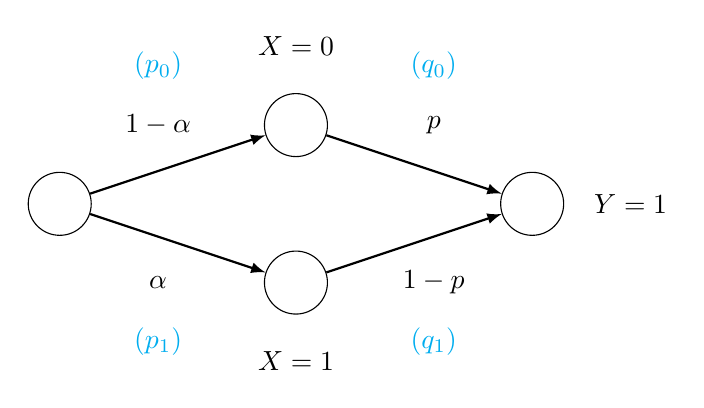
\begin{tikzpicture}[
      >=latex,
      node/.style={
        draw,circle,minimum size=0.8cm,inner sep=0pt
      },
    ]
    \node[node] (pr) at (0,0) {};
    \node[node] (x0) at (3,1) {};
    \node[node] (x1) at (3,-1) {};
    \node[node] (y1) at (6,0) {};
    \draw[thick,->] (pr) -- (x0);
    \draw[thick,->] (pr) -- (x1);
    \draw[thick,->] (x0) -- (y1);
    \draw[thick,->] (x1) -- (y1);
    \node[color=cyan] at (1.25,1.75) {$\left(p_0\right)$};
    \node[color=cyan] at (1.25,-1.75) {$\left(p_1\right)$};
    \node at (1.25,1) {$1-\alpha$};
    \node at (1.25,-1) {$\alpha$};
    \node[color=cyan] at (4.75,1.75) {$\left(q_0\right)$};
    \node[color=cyan] at (4.75,-1.75) {$\left(q_1\right)$};
    \node at (4.75,1) {$p$};
    \node at (4.75,-1) {$1-p$};
    \node at (3,2) {$X=0$};
    \node at (3,-2) {$X=1$};
    \node at (7.25,0) {$Y=1$};
  \end{tikzpicture}
\end{center}
\begin{equation*}
  \Rightarrow \MAP\left[X \mid Y=1\right] = \argmax_{i \in \{0,1\}}\ p_i q_i
.\end{equation*}
This yields the inequality statement,
\begin{equation*}
  p_0 q_0 \overset{\hat{X}_1=0}{\underset{\hat{X}_1=1}{\lessgtr}} p_1 q_1
\end{equation*}
where $\hat{X}_1$ is the $\MAP$ estimate of $X$ when $Y=1$ is $0$
or $1$. Thus
\begin{equation*}
  \left(1-\alpha\right) p\ \overset{0}{\underset{1}{\lessgtr}}\ \alpha \left(1-p\right)
\end{equation*}
